Significant progress has been made in the development of productive languages for concurrent computing. This section explores the desirable language requirements defined in Section \ref{feature}; examples of available languages are provided, along with insight into how they accomplish these requirements and how they inter-relate.

\subsection{Satisfying Reliability}
\label{sec:how:reliability}
% \comment{
%     Reo
%     Exogenous coordination language: you express the protocol in one place → it's easy to see if you program sticks to it. Facilitated by expressive features of the language
%     Rust
%     Implicit memory management with no runtime cost. Facilitated by expressive features of the language
%     Session types
%     Define the type of a communication channel to reflect protocol → compiler can ensure participants ahere
%     Modeling
%     mCRL2
% }
For a program to be reliable, it should perform its task consistently, as expected. Languages need to facilitate their programmers writing the code they intend to write. This simple goal has implications for a language's comprehensibility both for compilers (so that correctness can be definitively verified or errors identified) and humans (so that programs are written correctly in the first place).

\textbf{Reo}, \textbf{Manifold}, along with other exogenous communication languages provide this property in a way most languages do not: protocol code is located in one place~\cite{proper}. This isolation succeeds in more effectively capturing and preserving the \textit{intent} the programmer has in mind. Focusing on this idea of intent makes the mapping from the abstract algorithm to the Reo implementation easier and require less decision-making for the developer; additionally, it allows the problem to be expressed more coarsely, granting the compiler more freedom to optimize the details of the resulting binary. For example, Reo is able to perform \textit{protocol} optimizations such as merging distinct message channels onto one physical link~\cite{reoLinda}. Traditionally, \textit{actions} are first-class primitives and \textit{interactions} are derived concepts i.e. a message emerges from a \textit{send} and \textit{receive}; this spreads the interaction all over the source code.
Reo leans on the notion of upgrading \textit{interactions} to a first-class primitives instead~\cite{introReo}.

\textbf{Rust} is an imperative systems programming language with neither explicit memory management, nor a garbage collector. Its `ownership system' implements affine types, which requires that all data is associated with precisely one `owner' at a time, but may be `borrowed' (passed by reference) temporarily~\cite{rustSystem}. These borrows are gouverned by rules akin to those for the \textit{readers-writer lock}\footnote{The readers-writer lock is a concurrency mechanism for allowing multiple references without data races.}, requiring that no value is ever aliased and mutable at the same time. An example of the relationship between the ownership system and Rust syntax is given in Listing~\ref{lst:ownership}. This system prevents a program with dangling pointers or race conditions from compiling~\cite{patina}. Along with (optional) run-time array bounds-checking, this provides memory safety~\cite{rustbelt,patina}.
% DUMMY DUMMY DUMMY DUMMY DUMMY DUMMY DUMMY DUMMY DUMMY DUMMY DUMMY DUMMY DUMMY


\begin{listing}[t]
\footnotesize
\begin{minted}[breaklines,mathescape,frame=lines,tabsize=4]{rust}
fn foo(x: Data) { // foo consumes given x
	if bar() {
		let y = &mut x; // x aliased mutibly
	} // y goes out of scope
	baz(&x, &x); // x aliased with read-only refs
	// x references out of scope
} // x is dropped
\end{minted}
\caption{Illustration of the Rust ownership system (implementing affine types). References alias values with pointers until the references go out of scope. A mutable reference may not coexist with any other reference. Owned values that go out of scope are dropped implicitly.}
\label{lst:ownership}
\end{listing}

\textbf{Session types} are another paradigm for guaranteeing adherence to a communication protocol, often possible even at compile-time. In a nutshell, session types allow the programmer to express the type of a \textit{session} (representing a communication link) in a type system similar to that typically used for data types. Participants in the protocol can then only participate if the data they pass in or out is the correct type. Multi-party session types extend this notion to links with an arbitrary number of participants~\cite{sessionMultiparty}. Implementations for the various session type schemes either exist already or have been defined for languages Scribble, Rust, C, Erlang, Go, Java, Python, Scala and more~\cite{sessionRust,sessionHaskell}. Its wide adoption can be largely attributed the broad applicability of the concept. They can be implemented via libraries or natively, and checked statically or dynamically, etc. Consequently, languages without native support can be augmented by the addition of session types in a way that best suits the language.

\begin{listing}[t!]
\footnotesize
\begin{minted}[breaklines,mathescape,frame=lines,tabsize=4]{chapel}
config const m = 1000, alpha = 3.0;

const ProblemSpace = {0..m+1} dmapped Block(..), // allow algorithm to run on multiple locales. If unspecified, the domain maps on one locale only
      SubProblemSpace: subdomain(ProblemSpace) = {1..m}; 

var A, Temp: [ProblemSpace] real; // array of size ProblemSpace with elements of type real

//forall = concurrent alternative of for loop
A = alpha * A; // = forall a in A do alpha * a 
[i in SubProblemSpace] Temp[i] = (A[i-1] + A[i+1])/2; // = forall over SubProblemSpace indices
\end{minted}
\caption{Illustration of Chapel global view syntax. The code runs on multiple locales as the domain map was explicitly specified. The last two lines of code imply concurrent execution, each locale executes the code in parallel.}
\label{lst:globalView}
\end{listing}

Not only do we need the tools to create a reliable system, but we also need to be able to verify that it adheres to the protocol. This requires a good understanding of the execution semantics of our system. Analyzing models of the system's behaviour provides this understanding in a way that can be reproduced and easily communicated to others. However, modeling a complex concurrent system can be a challenging task, as was found by numerous sources ~\cite{modelConcurrentProblems,Fokkink2007ModellingDS, concurrentBMCModel}. The nature of exogenous coordination languages such as \textbf{Manifold} and \textbf{Reo} lends themselves well to graphical representations, making visual modelling of complex behavioral protocols a much easier task. For example, the authors of~\cite{model-reo} present a tool for converting Reo into mCRL2~\cite{mcrl2}. mCRL2 is a specification language that can be used to specify and analyze the behavior of distributed systems in Eclipse~\footnote{The most widely-used Java integrated development environment (IDE).}. Thanks to the user-friendly environment of mCRL2 in the Eclipse Coordination Tools (ECT), the implemented protocols can be visualized, verified and checked for correctness. In addition to validation, model-based checking easily maps to declarative models, reducing the gap between specification and implementation. This benefits developers as it is easier to maintain an overview of the implementation, as well as other non-technical stakeholders as they can more easily understand it.

%%%%%%%%%%%%%%%%%%%%%%%%%%%%%%%%%%%%%%%%%%%%%%%%
\subsection{Satisfying Productivity} \label{how:clarity}
% \comment{
%     Linda → manifold → Reo (graphical declarative langs)
%     They all aim 
%     Chapel
%     Impala
%     Transactional memory
%     how it interoperates with other langs
% }

Programming in a distributed setting is very challenging. It requires programmers to make the considerations inherent to sequential programming, with the added challenges of correct concurrency on top. Overcoming this difficulty requires the language to add minimal friction or risk overwhelming a programmer, leaving them unproductive~\cite{langNec}.

 \textbf{Transactional Memory} was introduced in the early 1990s to facilitate abstracting away from the tedious task of manually achieving mutual exclusion. Instead of locks, transactions allow multiple threads to initiate transactions in memory concurrently, keeping track of all read and write operations performed in the \textit{critical section}. Each thread \textit{commits} its changes when done, after which the transaction is irreversible. A check is first performed to determine if an involved memory location was modified by two threads; if so, the thread \textit{rolls back} the transaction, giving another thread an opportunity to commit~\cite{TMIntroduced}. Transactional memory is still an active area of research. However, the high cost of rollbacks inhibits its adoption as the primary solution to highly-concurrent applications~\cite{TMNotSolution}. Nevertheless, this type of abstraction was greatly appreciated by the development community, which still today utilizes transactional memory for specific purposes. We are still today working with the primitives that transactional memory tried to abstract away from, reflecting the necessity of another replacing language, tool or construct.

Where applicable, nothing achieves conciseness quite like a good abstraction. \textbf{Linda} manages to frame all communication operations in terms of four primitive actions on tuples, all variants of getting and setting tuples to and from a single persistent tuple store in the centralized, virtual shared memory `tuple space'~\cite{linda}. During development, Linda developers need only think in terms of these ubiquitous tuple operations, making it very easy to understand how the problem is being solved. It isn't until performance optimization becomes the priority that programmers have to look past the tuple abstraction. Even then, the compiler will do all the heavy lifting, distributing tuples between machines and optimizing ordering according to how they are accessed.

\textbf{Chapel} is a language that attempts to provide the benefits of a high-level global view approach to distributed programming (comparable to an exogenous coordination language) as well as the performance that sometimes requires fine control. At the higher levels, programs look more like pragma-augmented sequential code (familiar to developers that have worked with an OpenMP library), with specialized concurrent loops containing the data-parallel sections of code. An example of high-level global view Chapel can be seen in Listing~\ref{lst:globalView}. Whenever the higher levels differ from the programmer's needs in terms of data distribution, memory reuse etc., programmers can `dive down' to a lower layer, altering data distribution patterns or employing task parallelism~\cite{chapel}. This approach ensures Chapel code is only ever as complex as it needs to be, and granular details are present only because they represent deviations from the norm. 


% \begin{listing}[t!]
% \footnotesize
% \begin{minted}[breaklines,mathescape,frame=lines,tabsize=4]{chapel}
% config const m = 1000,
%       alpha = 3.0;

% const ProblemSpace = {0..m+1} dmapped Block(..), // allow algorithm to run on multiple locales. If unspecified, the domain maps on one locale only
%       SubProblemSpace: subdomain(ProblemSpace) = {1..m}; 

% var A, Temp: [ProblemSpace] real; // array of size ProblemSpace with elements of type real

% //forall = concurrent alternative of for loop
% A = alpha * A; // = forall a in A do alpha * a 
% [i in SubProblemSpace] Temp[i] = (A[i-1] + A[i+1])/2; // = forall over SubProblemSpace indices
% \end{minted}
% \caption{Illustration of Chapel global view syntax. The code runs on multiple locales as the domain map was explicitly specified. The last two lines of code imply concurrent execution, each locale executes the code in parallel.}
% \label{lst:globalView}
% \end{listing}

\textbf{Rust} offers a similar duality with `unsafe' code blocks. By marking a block with an explicit keyword, some operations that are not checked by Rust's ownership system are permitted~\cite{rustSystem}. This allows a programmer to explicitly manipulate raw pointers or statically type-cast values~\cite{patina}. The Rust community encourages the use of `pure safe rust', with popular libraries touting this safety in their doc pages. Unsafe Rust is used for cases where the compiler cannot be convinced of safety without turning to a sub-optimal formulation. Consider, for example, \textit{hogwild}, where threads write to a shared variable without locking, as the algorithm converges correctly regardless of arbitrary overwrites~\cite{hogwild}. The ownership system would prohibit these unsafe writes, as correctness cannot be inferred by the compiler~\cite{rustlang}.
%%%%%%%%%%%%%%%%%%%%%%%%%%%%%%%%%%%%%%%%%%%%%%%%%%%
\subsection{Satisfying Expressivity}
\label{sec:how:expressivity}

%A very small set of channels, each with very simple behavior, suffices to construct useful Reo connectors with significantly complex behavior. from proper

The architectural expressiveness of \textbf{Reo} make it well-suited for our purpose. The communication topology of components can be naturally established and described~\cite{criticalPathReo} making Reo accessible to developers. Figure~\ref{fig:reoArch} shows an example of an expressive communication model, a point-to-point model. Modifying one of the components make it easy to reason on how it may impact the other components~\cite{introReo}.
\begin{figure}
\centering
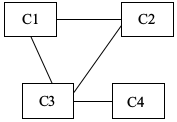
\includegraphics[page=1, width=0.25\textwidth]{images/reoArch.png}
\caption[h]{Architectural expressiveness. Communication pattern of a peer-to-peer model. The effect of modifying or replacing a component can be seen from this model, namely which other components will be affected. Image from~\cite{introReo}.}
\label{fig:reoArch}
\end{figure}
%Reo allows arbitrary user-defined channels as primitives; arbitrary mix of synchrony and asynchrony; and relational constraints between input and output. from proper

A study on the expressive power of Reo and Linda shows that the channel-based coordination model is surely more expressive as it allows mixing synchronous and asynchronous behaviour~\cite{reoLinda}.
For the same reason, Reo is considered more expressive than Manifold which only allows asynchronous behaviour~\cite{criticalPathReo}. 
Furthermore, Reo is more expressive than dataflow models, Kahn networks, synchronous languages, stream processing languages, workflow models and Petri nets~\cite{proper}.


% Chapel
Another prime example of an expressive language is \textbf{Chapel}. The global view programming model together with Chapel's language constructs for achieving data and task parallelism as described in Subsection \ref{how:clarity} represent principles that allow meaningful expression of real-world problems. 

Additionally, Chapel wishes to achieve interoperability with other languages such as C, to accommodate existing components~\cite{chapel}.
The support for calling between Chapel and C was already accomplished. Chapel is able to use external declaration of C concepts, i.e. functions, variables and types~\cite{chapelSite}.
At the time of writing, the interface with  C++, Java, Python, Fortran is in the process of being achieved through Babel, a high-performance language interoperability tool. Babel 2.0 includes an experimental version of Braid, which is an ongoing effort to support, among other languages, Chapel~\cite{babelSite}.

%%%%%%%%%%%%%%%%%%%%%%%%%%%%%%%%%%%%%%%%%%%%%%%%%%%%%
\subsection{Satisfying Performance}
\label{sec:how:performance}
% \comment{
%     Compilers do the dirty work
%     Reo and the sweet graph thingy
%     Rust compile time memory stuff
%     how it interoperates with other langs
% }
 

The ownership system of the \textbf{Rust} programming language, first outlined in Section~\ref{sec:how:reliability} and exemplified in Listing~\ref{lst:ownership}, is a purely compile-time construct. Rust is intended as a systems programming language; this incentivizes strong memory safety, while also necessitating competitive performance. While safe, the use of a garbage collector is prohibitively expensive. Instead, a Rust binary looks much like one created by a C compiler, with explicit allocation and de-allocation. These calls are inserted by the compiler at positions implicit by the structure of the source code~\cite{rustSystem}. Further language-integrations such as string slices allow generically-written iterator code without incurring run-time cost~\cite{slicing,vectorization}. This feature along with powerful and safe abstract macros\footnote{Macros in Rust are not based on string preprocessing. Rather, macros define operations on tokens in subtrees of the abstract syntax tree at compile time.} suit Rust well for the application of writing combinatory parsers for things like VLC Media Player's demuxers~\cite{rustParse,nom}.


% \begin{listing}[t]
% \footnotesize
% \begin{minted}[breaklines,mathescape,frame=lines,tabsize=4]{rust}
% fn foo(x: Data) { // foo consumes given x
% 	if bar() {
% 		let y = &mut x; // x aliased mutibly
% 	} // y goes out of scope
% 	baz(&x, &x); // x aliased with read-only refs
% 	// x references out of scope
% } // x is dropped
% \end{minted}
% \caption{Illustration of the Rust ownership system (implementing affine types). References alias values with pointers until the references go out of scope. A mutable reference may not coexist with any other reference. Owned values that go out of scope are dropped implicitly.}
% \label{lst:ownership}
% \end{listing}

\textbf{Impala} is a domain-specific dialect of Rust that seeks to take all of the syntax and much of the foundations of Rust to GPU programming. As with Rust, Impala leverages a novel, semantic-rich language extension to allow the compiler to optimize code extensively. Impala provides pragma\footnote{Pragmas are instructions in code that typically involve \textit{meta}-programming on other code constructs rather than mapping to anything in the binary; For example, inlining functions.}-like annotations which allow a compiler to evaluate some statements at compile-time, exploding control structures ahead of time; an example is provided in Listing~\ref{lst:partialEval}. Other instances generate code that exhibits `continuation-passing style', chaining functions together by passing subsequent code into functions as call arguments. These optimizations are exploited extensively by various GPU architectures, allowing further coalescing of task granularity for GPU threads. These features allow Impala to compile down to OpenGL and CUDA targets, making it portable while performing competitively~\cite{impala}.

\begin{listing}[t!]
\footnotesize
\begin{minted}[breaklines,mathescape,frame=lines,tabsize=4]{rust}
fn dot(a: &[i32], b: &[i32], n: i32) -> i32 {
    let mut sum = 0;
    for i in range(0, n) {
        sum += a(i) * b(i);
    }
    sum
}

fn main() -> i32 {
    let (a, b) = /* (omitted) */;
    let c = @dot(a, b, 4); // @ marks partial eval.
    
    /*  This generates:
    let mut c = 0;
    c += a(0) * b(0);
    c += a(1) * b(1);
    c += a(2) * b(2);
    c += a(3) * b(3);
	*/
}
\end{minted}
\caption{Example of an annotation in Impala resulting in partial evaluation of a function. Combined with normal compiler optimizations this results efficient GPU code. Source: \url{https://anydsl.github.io/Impala}.}
\label{lst:partialEval}
\end{listing}

\textsc{dream} is an aerodynamics application used to simulate the behaviour of fluids around moving bodies.
During the development, the authors report an extensive comparison between the message passing framework, PVM, and \textbf{Linda}~\cite{pvm, LindaVSMessage}. The evaluation is made on a cluster and both \textit{hardware performance} and \textit{elapsed time} are taken into consideration. The authors report consistent results of Linda outperforming PVM when scaling up the number of nodes and/or workload. This is mainly due to Linda's virtual shared memory system, offering automatic \textit{load balancing} capabilities in the tuple-space. This does not only allow for better scaling, but also requires less effort when developing. The results from the paper when running 9 compute nodes are visualized in Figure \ref{fig:pvmVsLinda}.

\begin{figure}[]
\centering
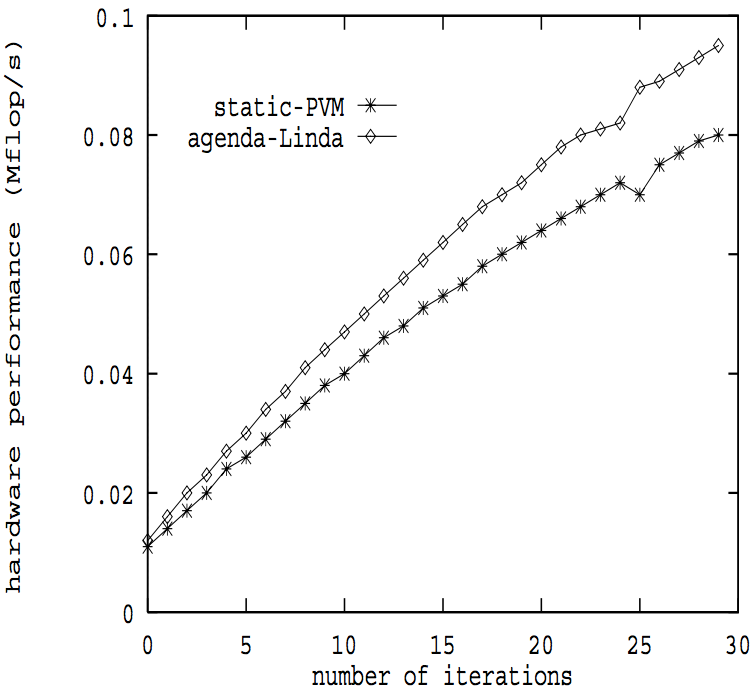
\includegraphics[page=1, width=0.45\textwidth]{images/pvmVsLinda.png}
\caption[]{Hardware performance of Linda and PVM applications for increasing number of time steps in the TDSL phase, using a 9-node multi-computer. Image from~\cite{LindaVSMessage}.}
\label{fig:pvmVsLinda}
\end{figure}

\textbf{Linda} outperforms PVM in scalability and execution speed. Furthermore, the authors stress that Linda was especially useful as `rapid application development platform', significantly decreasing the development time in comparison to PVM. Thanks to Linda's structure, the authors could perform different experiments by altering the coordination, a task which would take much more time in message passing framework due to its fine-grained structure. This case study shows how an abstract coordination language can be well-suited for the development of a complex distributed system containing many different tasks. Stitching components together is typically easier in a language that decouples process coordination and computation, since this provides a more easily maintained overview and more loosely coupled components. This holds also when using different programming languages~\cite{reoLinda}. As a result of their experience, the authors chose to continue to develop their system \textsc{dream}, with the tools offered by the Linda programming environment.

Despite its high-level approach, \textbf{Reo} has been shown to be capable of competing with hand-optimized C code. Reo is able to take the high-level protocol definition and apply \textit{protocol-level optimization} (deduplicating communication links, etc.) during compilation. Even more importantly, Reo is capable of leveraging the \textit{Proto-Runtime-Toolkit} (PRT) for all its granular concurrency primitives. PRT offers control over system resources \textit{without} involvement of the OS scheduler~\cite{proper}; Figure \ref{fig:reoPerf} illustrates this positive result. Arbab et al. argue that many imperative languages cannot hope to meaningfully compile down to PRT the way Reo does, as the languages are too fine-grained for the compilers to be able to effectively map native source code to PRT. PRT is far too platform-specific and low-level for any programmer to interact with productively for any implementation of realistic complexity. They summarize this sentiment in Figure~\ref{fig:actInter}; for the imperative example, the large effort of the programmer is illustrated by the large `distance' from the high-level declarative algorithm to the low-level imperative implementation in a traditional language. The corresponding compiler has little room to apply optimizations as the code it is provided with is already highly specified. By contrast, the Reo-approach affords a smaller step from algorithm to implementation by the programmer, relegating more granular work to the compiler. For this reason, the compiler is at liberty to perform optimizations at the protocol level as well as those used in both cases to make best use of the quirks of the target machine (cache coherence, etc.). Arbab et al. recognize that in both cases optimizations are performed, but in the latter case, they are performed by the less error-prone \textit{compiler} rather than a human~\cite{proper}.

\begin{figure}
\centering
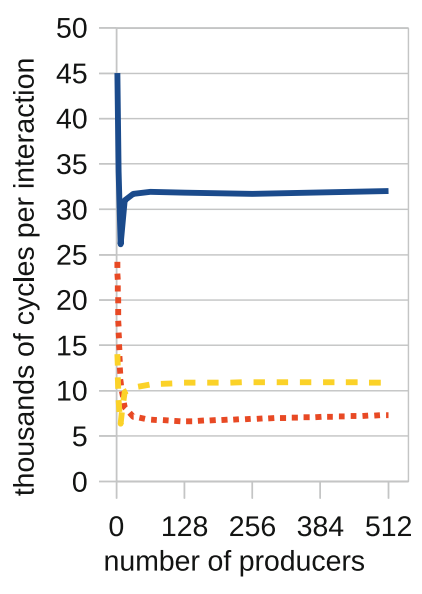
\includegraphics[page=1, width=0.27\textwidth]{images/reoPerf.png}
\caption[]{CPU cycles per interaction for N-Producer-1-Consumer implementation with na\"{i}ve C implementation in solid navy, hand-optimized C implementation in dashed yellow and Reo in dotted red.. Image from~\cite{proper}.}
\label{fig:reoPerf}
\end{figure}


\begin{figure}
\centering
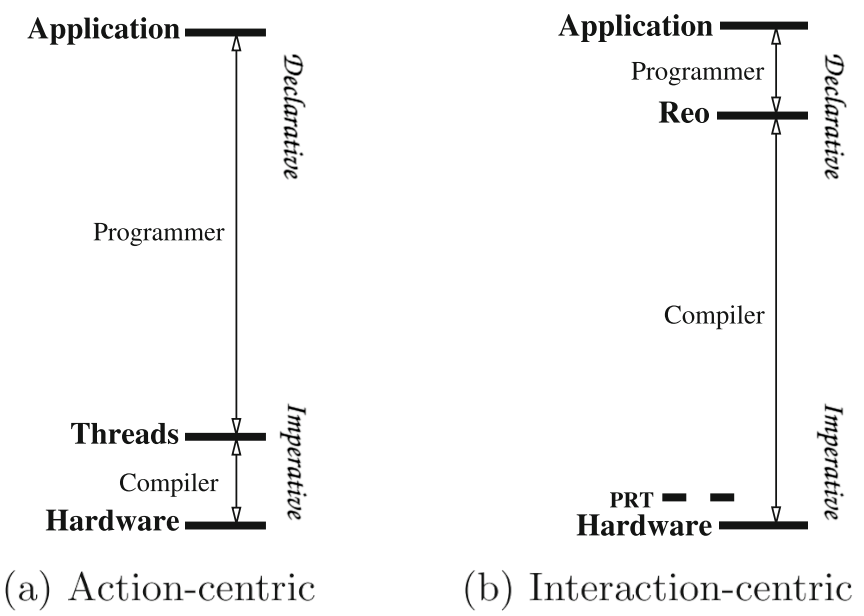
\includegraphics[page=1, width=0.46\textwidth]{images/actInter.png}
\caption[]{Visualization of the transformations necessary from the abstract algrithm to the ultimate imperative machine code for (a) a traditional, imperative language like C (b) Reo. Image from~\cite{proper}.}
\label{fig:actInter}
\end{figure}


% \begin{figure}
% \centering
% 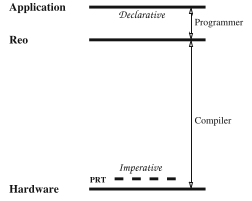
\includegraphics[page=1, width=0.4\textwidth]{images/interaction.png}
% \caption[]{Visualization of the transformations necessary from the abstract algrithm to the ultimate imperative machine code, in this case for Reo. Image from~\cite{proper}.}
% \label{fig:interaction}
% \end{figure}


